% ============================================================================
% ACM/IEEE Design Automation Conference (DAC) Submission Manuscript
% ----------------------------------------------------------------------------
% DAC REQUIREMENTS:
%   - Format: Standard IEEE double-column conference format (US Letter)
%   - Strict Double-Blind Review: \anonymoustrue (zero author/affiliation identifiers)
%   - Page Limit: Hard 6.0-page limit for technical text, figures, and tables,
%                 plus up to 1 additional page containing exclusively references.
% ============================================================================
\newif\ifanonymous
\anonymoustrue
% \anonymousfalse

\documentclass[conference]{IEEEtran}
\IEEEoverridecommandlockouts

\usepackage{cite}
\usepackage{amsmath,amssymb,amsfonts,bm}
\usepackage{algorithm}
\usepackage{algorithmic}
\usepackage{graphicx}
\usepackage{booktabs}
\usepackage{multirow}
\usepackage{array}
\usepackage{xcolor}
\usepackage{url}
\usepackage{microtype}

\graphicspath{{./figures/}}

% IEEE/DAC-compliant float & caption spacing for compact publication
\renewcommand{\topfraction}{0.92}
\renewcommand{\dbltopfraction}{0.92}
\renewcommand{\bottomfraction}{0.85}
\renewcommand{\textfraction}{0.06}
\renewcommand{\floatpagefraction}{0.85}
\renewcommand{\dblfloatpagefraction}{0.85}
\setlength{\textfloatsep}{5pt plus 2pt minus 2pt}
\setlength{\dbltextfloatsep}{5pt plus 2pt minus 2pt}
\setlength{\floatsep}{4pt plus 2pt minus 2pt}
\setlength{\dblfloatsep}{4pt plus 2pt minus 2pt}
\setlength{\abovecaptionskip}{2.0pt plus 1pt minus 1pt}
\setlength{\belowcaptionskip}{0.5pt}
\AtBeginDocument{%
  \setlength{\abovedisplayskip}{3.5pt plus 1.0pt minus 1.0pt}%
  \setlength{\belowdisplayskip}{3.5pt plus 1.0pt minus 1.0pt}%
  \setlength{\abovedisplayshortskip}{2.0pt plus 1.0pt minus 1.0pt}%
  \setlength{\belowdisplayshortskip}{2.5pt plus 1.0pt minus 1.0pt}%
}

\renewcommand{\algorithmicrequire}{\textbf{Input:}}
\renewcommand{\algorithmicensure}{\textbf{Output:}}
\renewcommand{\algorithmiccomment}[1]{~~$\triangleright$~{\itshape #1}}

\begin{document}

\title{Breaking the Memory and Communication Walls of Distributed Complex GEMM on Multi-Zone Heterogeneous DSP Supercomputers}

\ifanonymous
\author{\IEEEauthorblockN{Anonymous Author(s)}
\IEEEauthorblockA{\textit{Design Automation Conference (DAC) Blind Review Submission}}}
\else
\author{\IEEEauthorblockN{First A. Author\IEEEauthorrefmark{1}, Second B. Author\IEEEauthorrefmark{1}, and Third C. Author\IEEEauthorrefmark{2}}
\IEEEauthorblockA{\IEEEauthorrefmark{1}\textit{College of Computer Science and Technology, National Key Laboratory of Parallel and Distributed Computing}\\
Email: \{author1, author2\}@institution.edu}
\IEEEauthorblockA{\IEEEauthorrefmark{2}\textit{National Supercomputing Center}\\
Email: author3@nscc.edu}}
\fi

\maketitle

\begin{abstract}
Double-precision complex general matrix-matrix multiplication (ZGEMM) is foundational to computational electromagnetics, quantum chemistry, and dense linear algebra solvers in electronic design automation (EDA). Deploying large-scale ZGEMM on multi-zone heterogeneous supercomputers---exemplified by the MT-3000 processor coupling 16 ARMv8 cores with four autonomous 24-core bare-metal VLIW/SIMD DSP clusters per node---reveals two primary constraints: on-chip scratchpad bandwidth saturation without hardware caches, and inter-node collective communication serialization across thousands of accelerator processes.

We present an end-to-end hardware-software co-design framework addressing both memory and network bottlenecks. At the intra-chip level, we architect a 14-channel asynchronous DMA tri-buffered scratchpad pipeline ($C$-matrix cyclic triple buffering nested around $A/B$ ping-pong double buffering) paired with a $4 \times 4$ register-resident dual-FMA micro-kernel that pins 32 physical 16-lane FP64 vector accumulators, eliminating $86.1\%$ ($7.20\times$) of Array Memory vector traffic. At the inter-node level, we formulate a Stationary-$A$, Panel-Broadcast-$B$ 2D hybrid orchestration ($P/2 \times 2$) incorporating zero-copy strided panel extraction via committed \texttt{MPI\_Type\_vector} datatypes, two-phase non-blocking subgroup collectives, offset-addressed parallel POSIX \texttt{pread} directly into DSP-mapped memory overlapped with network transfers, and 64-column vector-aligned intra-cluster partitioning. On single-node benchmarks ($N=512$ to $16384$), 1 DSP core sustains $49.19$~GFLOPS ($64.1\%$ of dual-FMA peak; $6.12\times$--$7.28\times$ over OpenBLAS), 1 cluster reaches $243.44$~GFLOPS ($\sim\!100\%$ of the $240.5$~GFLOPS DDR4 DMA Roofline; $9.33\times$ over 4-core CPU), and 1 full node reaches $956.17$~GFLOPS with FP64 $\ell_\infty$ error $\le 2.18 \times 10^{-8}$. Scaling across 512 MT-3000 nodes (2,048 MPI processes, 49,152 DSP cores), our co-design reduces $8192^3$ collective time by $9.90\times$ ($102.25 \to 10.32$~s), halves the DDR-streaming floor to $89.92$~TFLOPS ($2.01\times$ over 1D), scales extreme $16384^3$ workloads to $218.79$~TFLOPS ($222.49\times$ speedup, $112.80\%$ 2-node superlinear efficiency), and maintains $92.21\%$ weak-scaling efficiency at 49,152 DSP cores.
\end{abstract}

\begin{IEEEkeywords}
Complex GEMM (ZGEMM), multi-zone processor, MT-3000 DSP, scratchpad memory (SPM), asynchronous DMA triple buffering, 2D hybrid MPI collectives, Roofline model.
\end{IEEEkeywords}

% ============================================================================
\section{Introduction}
\label{sec:intro}
% ============================================================================
Double-precision complex general matrix-matrix multiplication (ZGEMM), defined for split-complex matrices $A \in \mathbb{C}^{M \times K}$, $B \in \mathbb{C}^{K \times N}$, and $C \in \mathbb{C}^{M \times N}$ as $C \leftarrow C + AB$, is a foundational computational building block in high-frequency computational electromagnetics, quantum chemistry, radar imaging, and complex matrix solvers in electronic design automation (EDA)~\cite{barrett2010complexhpl, vanzee2017complex}. Unlike real DGEMM ($2MNK$ FLOPs), ZGEMM requires $8MNK$ double-precision operations---four real matrix multiplications and four real matrix additions/subtractions---imposing quadrupled arithmetic density and doubled memory footprints.

To address power and energy walls, modern high-performance processors increasingly substitute hardware cache hierarchies with software-managed scratchpad memories (SPMs) and explicit direct memory access (DMA) engines~\cite{kahle2005cell, igual2012dsp, fu2016sunway, jiang2017sw26010}. The \textbf{MT-3000} multi-zone processor~\cite{lu2022mt3000} exemplifies this architectural paradigm, coupling a 16-core ARMv8 General-Purpose (GP) Zone with a 96-core Acceleration (ACC) Zone partitioned into four autonomous 24-core bare-metal VLIW/SIMD DSP clusters ($11.6$~TFLOPS node peak at $1.2$~GHz). Each DSP core integrates a $64$~KB Scalar Memory (SM) and a $768$~KB vector Array Memory (AM), with no hardware cache to off-chip DDR4~\cite{fang2026mtgemm, qi2025constraint}.

While prior work has accelerated real-valued kernels on single MT-3000 nodes~\cite{fang2026mtgemm, mo2024irregular, qi2025constraint, qi2026attention}, scaling distributed complex ZGEMM across hundreds of heterogeneous nodes exposes four coupled challenges:
\begin{enumerate}\setlength{\itemsep}{0.5pt}\setlength{\parskip}{0pt}
    \item \textbf{Complex Register Pressure and AM Traffic Amplification:} Updating real ($C_{\mathrm{Re}}$) and imaginary ($C_{\mathrm{Im}}$) tiles involves four coupled cross-terms. Naive inner-loop accumulation from AM ($2{,}304$ vector memory ops per $4 \times 64 \times 32$ block) starves dual-issue fused multiply-add (FMA) units, whereas algebraic 3M reductions~\cite{vanzee2017complex} demand auxiliary memory and induce $\mathcal{O}(\kappa)$ numerical cancellation~\cite{higham2002accuracy}.
    \item \textbf{Asymmetric Scratchpad Capacity and Exposed $C$-Tile DMA:} All active $A$, $B$, and $C$ buffers must co-reside inside $64$~KB SM and $768$~KB AM. Standard $A/B$ ping-pong double buffering hides inner $K$-loop fetches but leaves bidirectional DDR4$\leftrightarrow$AM load and write-back latencies of $C$ exposed at outer tile boundaries.
    \item \textbf{Supercomputer-Scale Collective Contention and Serialized Root I/O:} Binding one MPI rank per autonomous DSP cluster creates $2{,}048$ ranks across $512$ nodes. Globally broadcasting a $1.074$~GB complex $B$ matrix ($8192^2 \times 16$~B) incurs severe interconnect contention ($102.25$~s at 512 nodes---over $1{,}040\times$ the kernel compute time), while root-serialized storage reads leave $2{,}047$ clusters idle.
    \item \textbf{Strong-Scaling Off-Chip DDR-Streaming Floor:} Under strong scaling ($N=8192$), once per-cluster row height $M_{\mathrm{local}}$ drops below scratchpad tile height $M_b = 56$ ($P > 146$ in 1D), arithmetic intensity collapses from $14.83$ to $1.88$~FLOPs/Byte, locking 1D execution to a hard DDR4 streaming floor ($0.0982$~s, $44.78$~TFLOPS).
\end{enumerate}

To overcome these constraints simultaneously, we present a full-stack hardware-software co-design:
\begin{itemize}\setlength{\itemsep}{0.5pt}\setlength{\parskip}{0pt}
    \item \textbf{14-Channel Tri-Buffered Pipeline and $4 \times 4$ Micro-Kernel:} We coordinate 14 hardware P2P DMA channels to nest inner $A/B$ ping-pong double buffering ($56$~KB SM + $64$~KB AM) inside middle $C$-matrix cyclic triple buffering ($168$~KB AM). Our $4 \times 4$ micro-kernel pins 32 physical 16-lane FP64 vector registers across $K_b=32$ steps using hoisted SPU negation and \texttt{vec\_svbcast}, cutting AM traffic by $86.1\%$ ($7.20\times$).
    \item \textbf{Stationary-$A$, Panel-Broadcast-$B$ 2D Orchestration ($P/2 \times 2$):} We eliminate network transfers of $A$ and post-compute reductions of $C$ via disjoint 2D output ownership, zero-copy strided panel dispatch via committed \texttt{MPI\_Type\_vector} types, two-phase non-blocking subgroup collectives overlapped with concurrent POSIX \texttt{pread}, and 64-column vector-aligned intra-cluster partitioning, analytically proving the optimality of $G=2$.
    \item \textbf{Capacity Proof and Strong-Scaling DDR-Floor Theorem:} We establish a closed-form scratchpad capacity model proving that tile $(56, 32, 64)$ achieves $\mathcal{I}_{\mathrm{DMA}} = 14.83$~FLOPs/Byte ($240.5$~GFLOPS cluster DDR ceiling), and derive the strong-scaling streaming floor theorem predicting a $2.0\times$ asymptotic kernel speedup at scale.
    \item \textbf{Multi-Scale 1- to 512-Node Supercomputer Validation:} Our kernel achieves $49.19$~GFLOPS/core ($64.1\%$ peak; $6.12\times$--$7.28\times$ over OpenBLAS), $243.44$~GFLOPS/cluster ($\sim\!100\%$ Roofline), and $956.17$~GFLOPS/node. Across 512 nodes (49,152 DSP cores), our co-design cuts $8192^3$ collective time by $9.90\times$, doubles kernel throughput to $89.92$~TFLOPS ($2.01\times$ over 1D), reaches $218.79$~TFLOPS at $16384^3$ ($222.49\times$ speedup, $112.80\%$ 2-node superlinear efficiency), and sustains $92.21\%$ weak-scaling efficiency.
\end{itemize}

% ============================================================================
\section{Architectural Background \& Machine Balance}
\label{sec:background}
% ============================================================================

\subsection{MT-3000 Multi-Zone Architecture and Scratchpads}
As illustrated in Fig.~\ref{fig:arch} and detailed in Table~\ref{tab:hw_specs}, the MT-3000 processor adopts a heterogeneous multi-zone SoC architecture~\cite{lu2022mt3000}. The \emph{GP Zone} comprises 16 ARMv8 CPU cores running Linux and the MPI runtime. The \emph{ACC Zone} integrates four physically autonomous DSP clusters managed via the lightweight \texttt{Hthread} driver. Because each DSP cluster maintains independent command queues, on-chip shared memories, and DMA controllers without inter-cluster cache coherence, we bind one MPI rank exclusively to each DSP cluster ($\mathrm{dev\_id} = \mathrm{rank} \bmod 4$, 4 ranks/node), eliminating intra-node device contention.

\begin{figure}[t]
    \centering
    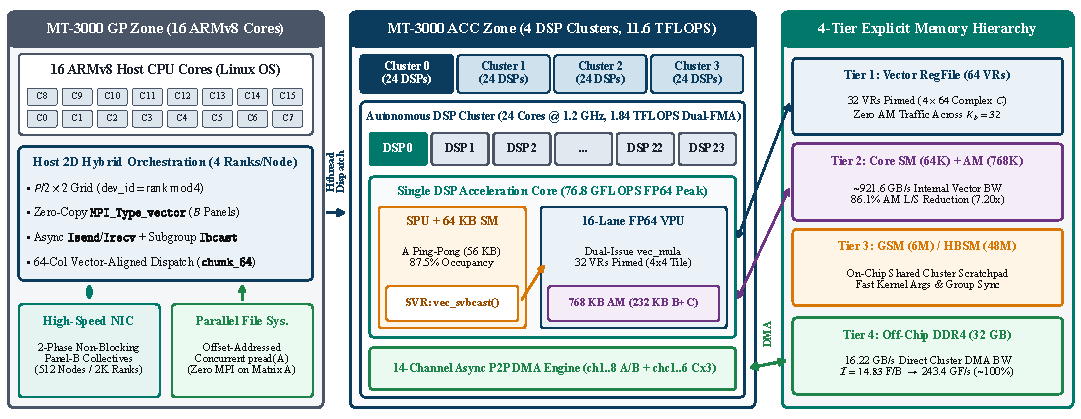
\includegraphics[width=\columnwidth]{fig1_arch_overview.pdf}
    \caption{MT-3000 multi-zone heterogeneous node architecture, 4-tier SPM hierarchy, and mapping of our ZGEMM co-design across ARMv8 and DSP clusters.}
    \label{fig:arch}
\end{figure}

\begin{table}[t]
\centering
\caption{Verified Specifications of an MT-3000 Node~\cite{lu2022mt3000, qi2025constraint}}
\label{tab:hw_specs}
\renewcommand{\arraystretch}{1.06}
\setlength{\tabcolsep}{3.0pt}
\resizebox{\columnwidth}{!}{%
\begin{tabular}{@{}lll@{}}
\toprule
\textbf{Zone / Tier} & \textbf{Parameter} & \textbf{Verified Specification} \\
\midrule
GP Zone & Host CPU Cores & 16 ARMv8 Cores (Linux OS; 4 Ranks/Node) \\
\midrule
\multirow{4}{*}{ACC Zone} & DSP Clusters / Cores & 4 Clusters/Node (1/Rank); 24 Cores/Cluster (96C/Node) \\
 & Clock Frequency & 1.2 GHz; 1,536 FP64 VPU Lanes/Node \\
 & Compute Peak & 76.8 GF/s per Core; 1.84 TF/s per Cluster; 11.6 TF/s Node \\
 & DDR4 DMA BW & 32 GB Shared DDR4; \textbf{16.22 GB/s} Cluster Direct DMA \\
\midrule
\multirow{3}{*}{4-Tier Memory} & Vector Regs (VR) & 64 $\times$ 1,024-bit ($16 \times$ FP64) per Core \\
 & Scalar Mem (SM) & 64 KB per Core (SPU control + \texttt{vec\_svbcast}) \\
 & Array Mem (AM) & 768 KB per Core ($\sim$921.6 GB/s wide vector access) \\
\bottomrule
\end{tabular}%
}
\end{table}

Each DSP cluster houses 24 bare-metal DSP cores clocked at $1.2$~GHz. Within each core, a Scalar Processing Unit (SPU) accesses private $64$~KB \emph{Scalar Memory (SM)} and broadcasts scalar operands via \texttt{vec\_svbcast}. A coupled 16-lane FP64 Vector Processing Unit (VPU) features 64 physical 1,024-bit vector registers (\texttt{lvector double}) and dual-issue FMA pipelines (\texttt{vec\_mula}), delivering a theoretical vector peak:
\begin{equation}
\mathcal{P}_{\mathrm{core}} = 16 \times 2\,\text{FMA} \times 2\,\text{FLOPs} \times 1.2\,\text{GHz} = 76.8\,\text{GFLOPS},
\label{eq:core_peak}
\end{equation}
yielding $\mathcal{P}_{\mathrm{cluster}} = 1{,}843.2$~GFLOPS per 24-core cluster. The VPU executes wide vector loads/stores (\texttt{vec\_ld}/\texttt{vec\_st}) exclusively against its private $768$~KB \emph{Array Memory (AM)} at $\sim\!921.6$~GB/s. Because no hardware cache exists between off-chip DDR4 and SM/AM, all data movement must be explicitly scheduled in software via point-to-point hardware DMA channels (\texttt{dma\_p2p}), with measured direct cluster DMA bandwidth $\mathcal{B}_{\mathrm{DDR}} = 16.22$~GB/s~\cite{qi2025constraint}.

\subsection{Split-Complex Planar Format vs.\ Algebraic 3M}
For split-complex matrices $A = A_{\mathrm{Re}} + i A_{\mathrm{Im}}$, $B = B_{\mathrm{Re}} + i B_{\mathrm{Im}}$, and $C = C_{\mathrm{Re}} + i C_{\mathrm{Im}}$, ZGEMM computes:
\begin{equation}
\begin{aligned}
C_{\mathrm{Re}} &\leftarrow C_{\mathrm{Re}} + A_{\mathrm{Re}} B_{\mathrm{Re}} - A_{\mathrm{Im}} B_{\mathrm{Im}}, \\
C_{\mathrm{Im}} &\leftarrow C_{\mathrm{Im}} + A_{\mathrm{Re}} B_{\mathrm{Im}} + A_{\mathrm{Im}} B_{\mathrm{Re}}.
\end{aligned}
\label{eq:zgemm_4m}
\end{equation}
Standard Array-of-Structures (AoS) complex layouts ($[x_0, y_0, \dots]$) force costly in-register shuffling on 16-lane VPUs lacking de-interleaving crossbars. We adopt \emph{split-complex planar} (SoA) layout, aligning 16 consecutive real or imaginary elements directly to 128-byte \texttt{vec\_ld} operations. Furthermore, while Gauss 3M methods reduce operations to $6MNK$ FLOPs~\cite{vanzee2017complex}, they consume auxiliary DDR4 buffers and suffer $\mathcal{O}(\kappa)$ numerical cancellation~\cite{higham2002accuracy}. We execute exact 4M accumulation via native dual-issue \texttt{vec\_mula} instructions, preserving FP64 accuracy without workspace allocation.

\subsection{Machine Balance and the Scratchpad Memory Wall}
Dividing cluster peak $\mathcal{P}_{\mathrm{cluster}} = 1{,}843.2$~GFLOPS by off-chip bandwidth $\mathcal{B}_{\mathrm{DDR}} = 16.22$~GB/s exposes a steep machine balance ridge point~\cite{williams2009roofline}:
\begin{equation}
\mathcal{I}_{\mathrm{ridge}} = \mathcal{P}_{\mathrm{cluster}} / \mathcal{B}_{\mathrm{DDR}} = 1{,}843.2 / 16.22 = 113.64\,\text{FLOPs/B}.
\label{eq:ridge}
\end{equation}
For a complex tile $(M_b, K_b, N_b)$ in $64$~KB SM and $768$~KB AM, transferring $16(M_b K_b + K_b N_b)$ bytes to perform $8 M_b K_b N_b$ FLOPs bounds arithmetic intensity to $\mathcal{I}_{\max} < \frac{M_b N_b}{2(M_b + N_b)}$. Even if $A$ occupied the entire $64$~KB SM ($M_b \approx 64$), $\mathcal{I}_{\max} \le 16$~FLOPs/B $\ll 113.64$~FLOPs/B. Thus, \emph{multi-core ZGEMM is fundamentally DDR4-DMA-bound at the cluster level, yet AM-port- and FMA-latency-bound within each core}. Maximizing performance requires saturating tile arithmetic intensity while fully overlapping DDR4 DMA with VPU execution.

\begin{figure*}[t]
    \centering
    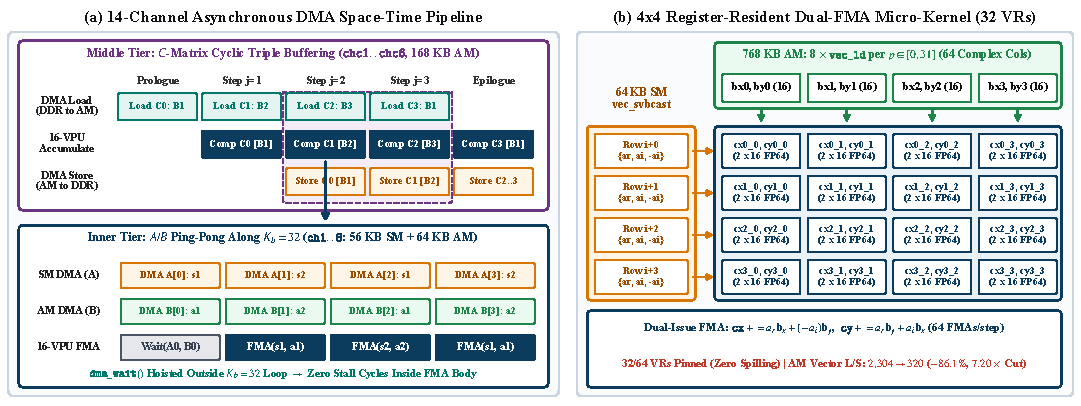
\includegraphics[width=0.68\textwidth]{fig3_tri_pipeline_microkernel.pdf}
    \caption{Intra-chip scratchpad and register co-design: (a) 14-channel asynchronous DMA space-time pipeline nesting inner $A/B$ double buffering inside middle $C$ cyclic triple buffering; (b) $4 \times 4$ register-resident dual-FMA micro-kernel pinning 32 vector accumulators to cut AM traffic by $86.1\%$.}
    \label{fig:microkernel}
\end{figure*}

% ============================================================================
\section{Tri-Buffered Scratchpad Pipeline \& Micro-Kernel}
\label{sec:device}
% ============================================================================

\subsection{14-Channel Asynchronous DMA Tri-Buffered State Machine}
On cacheless DSP cores, conventional $A/B$ ping-pong double buffering leaves the bidirectional DDR4 read and write-back latencies of each $M_b \times N_b$ complex $C$ tile ($112$~KB round-trip) unhidden between $K$-reductions. We resolve this via a \textbf{14-channel two-tier DMA state machine} (\texttt{kernel\_pipeline.c}; Fig.~\ref{fig:microkernel}(a) and Algorithm~\ref{alg:device_kernel}):
\begin{enumerate}\setlength{\itemsep}{0.5pt}\setlength{\parskip}{0pt}
    \item \textbf{Middle-Tier $C$ Cyclic Triple Buffering (6 Channels, \texttt{chc1..chc6}):} Three split-complex buffer pairs reside in AM ($168$~KB total). Cyclic rotation maps buffer $(j/N_b) \bmod 3$ to prefetch $C^{(j)}$ via strided DMA, buffer $(j/N_b - 1) \bmod 3$ to active VPU $K$-accumulation, and buffer $(j/N_b - 2) \bmod 3$ to asynchronous DDR4 write-back of $C^{(j-2N_b)}$, hiding $100\%$ of bidirectional $C$ DMA traffic behind compute.
    \item \textbf{Inner-Tier $A/B$ Ping-Pong Double Buffering (8 Channels, \texttt{ch1..ch8}):} Two complex $A$ pairs reside in $64$~KB SM (\texttt{ch1..ch4}, $56$~KB); two complex $B$ pairs reside in $768$~KB AM (\texttt{ch5..ch8}, $64$~KB). Non-blocking prefetches for step $k+K_b$ are posted before compute on step $k$, hoisting all \texttt{dma\_wait} barriers outside the inner $K_b=32$ FMA loop.
\end{enumerate}

\begin{algorithm}[t]
\caption{Device-Side 14-Channel Tri-Buffered DSP Kernel}
\label{alg:device_kernel}
\footnotesize
\begin{algorithmic}[1]
\REQUIRE $A \in \mathbb{C}^{M_r \times K}, B \in \mathbb{C}^{K \times N_g}, C \in \mathbb{C}^{M_r \times N_g}$; core $t \in [0, 23]$; $(M_b, K_b, N_b) = (56, 32, 64)$.
\ENSURE Updated core slice $C[:, j_0(t) : j_0(t)+N_{\mathrm{thread}}(t)]$.
\STATE Allocate SM ping-pong $A_{1,2}$ ($56$~KB), AM ping-pong $B_{1,2}$ ($64$~KB), AM triple $C_{1..3}$ ($168$~KB).
\FOR{$i = 0$ \TO $M_r - 1$ \textbf{step} $M_b$}
    \STATE Async \texttt{dma\_p2p} load $C[i, j_0] \to C_1$.
    \FOR{$j = N_b$ \TO $N_{\mathrm{thread}}(t) - 1$ \textbf{step} $N_b$}
        \STATE Rotate $(s_{\mathrm{store}}, s_{\mathrm{comp}}, s_{\mathrm{load}}) \bmod 3$; post async prefetch $C[i, j_0+j] \to C_{s_{\mathrm{load}}}$.
        \STATE Post async $A[i, 0] \to A_1$, $B[0, j_0+j-N_b] \to B_1$; wait on $C_{s_{\mathrm{comp}}}$ and prior $C_{s_{\mathrm{store}}}$.
        \FOR{$k_{\mathrm{idx}} = 0$ \TO $\lceil K / K_b \rceil - 1$}
            \STATE $b \leftarrow (k_{\mathrm{idx}} \bmod 2) + 1$; $\bar{b} \leftarrow 3 - b$.
            \IF{$k_{\mathrm{idx}} + 1 < \lceil K / K_b \rceil$}
                \STATE Post async prefetch $A_{k+K_b} \to A_{\bar{b}}$ and $B_{k+K_b} \to B_{\bar{b}}$.
            \ENDIF
            \STATE \texttt{dma\_wait} on $(A_b, B_b)$; load 32 VRs $\{\mathbf{cx}_{u,v}, \mathbf{cy}_{u,v}\}$ from $C_{s_{\mathrm{comp}}}$.
            \FOR{$p = 0$ \TO $K_b - 1$}
                \STATE Load 8 vectors $B$ from $B_b$; broadcast $\{a_r, a_i, -a_i\}$; execute dual \texttt{vec\_mula}.
            \ENDFOR
            \STATE Store 32 VRs to $C_{s_{\mathrm{comp}}}$.
        \ENDFOR
        \STATE Post async \texttt{dma\_p2p} store $C_{s_{\mathrm{comp}}} \to C[i, j_0+j-N_b]$.
    \ENDFOR
    \STATE Finalize remaining tile accumulation and await DMA write-back completion.
\ENDFOR
\end{algorithmic}
\end{algorithm}

\subsection{$4 \times 4$ Vector-Register-Resident Dual-FMA Micro-Kernel}
Naive inner-loop accumulation from AM issues $2{,}304$ vector memory operations for $2{,}048$ FMAs ($0.89$ FMAs/access), causing severe port contention. We design a \textbf{$4 \times 4$ outer-product micro-kernel} (Fig.~\ref{fig:microkernel}(b)):
\begin{itemize}\setlength{\itemsep}{0.5pt}\setlength{\parskip}{0pt}
    \item \textbf{32-VR Accumulator Pinning (Zero Spilling):} We unroll 4 rows along $M_b$ and 4 vector segments ($4 \times 16 = 64$ columns) along $N_b$, pinning $4 \times 4 \times 2 = \mathbf{32}$ physical vector registers ($\mathbf{cx}_{u,v}, \mathbf{cy}_{u,v}$) for the $C$ sub-tile. With 8 streaming $B$ registers and 3 broadcast $A$ registers, total live register count is 43 of 64 VRs ($67.2\%$), guaranteeing zero compiler spilling to AM.
    \item \textbf{Hoisted SPU Negation for Dual-Issue \texttt{vec\_mula}:} For each row, the SPU computes $-a_i$ in scalar arithmetic and broadcasts $\{a_r, a_i, -a_i\}$ via \texttt{vec\_svbcast}, enabling all 32 real and 32 imaginary updates per step to execute exclusively as fused dual-issue \texttt{vec\_mula} instructions without subtract instructions:
    \begin{equation}
    \begin{aligned}
    \mathbf{cx}_{u,v} &\leftarrow \texttt{vec\_mula}(\tilde{\mathbf{a}}_{r,u},\, \mathbf{bx}_v,\, \mathbf{cx}_{u,v}), \\
    \mathbf{cx}_{u,v} &\leftarrow \texttt{vec\_mula}(-\tilde{\mathbf{a}}_{i,u},\, \mathbf{by}_v,\, \mathbf{cx}_{u,v}), \\
    \mathbf{cy}_{u,v} &\leftarrow \texttt{vec\_mula}(\tilde{\mathbf{a}}_{r,u},\, \mathbf{by}_v,\, \mathbf{cy}_{u,v}), \\
    \mathbf{cy}_{u,v} &\leftarrow \texttt{vec\_mula}(\tilde{\mathbf{a}}_{i,u},\, \mathbf{bx}_v,\, \mathbf{cy}_{u,v}).
    \end{aligned}
    \label{eq:vec_mula}
    \end{equation}
    \item \textbf{$86.1\%$ AM Traffic Elimination:} Vectors $\mathbf{cx}_{u,v}, \mathbf{cy}_{u,v}$ are loaded once before $p=0$ and stored once after $p=31$. Total AM instructions drop from $2{,}304$ to $32 + 256 + 32 = \mathbf{320}$ ($7.20\times$ fewer accesses), raising arithmetic density to $64 / 8 = \mathbf{8.0}$ vector FMAs per vector load.
\end{itemize}

\subsection{Scratchpad Capacity Proof and Strong-Scaling Streaming Floor}
Selecting $(M_b, K_b, N_b)$ is constrained by SM ($64$~KB) and AM ($768$~KB):
\begin{equation}
\begin{aligned}
\mathcal{S}_{\mathrm{SM}} &= 4 M_b K_b \times 8\,\text{B} \le 56\,\text{KB}, \\
\mathcal{S}_{\mathrm{AM}} &= (4 K_b N_b + 6 M_b N_b) \times 8\,\text{B} \le 768\,\text{KB}.
\end{aligned}
\label{eq:capacity}
\end{equation}
Fixing $N_b = 64$ and $K_b = 32$,~\eqref{eq:capacity} yields optimal $M_b = 56$ ($56 = 14 \times 4$), using $\mathcal{S}_{\mathrm{SM}} = \mathbf{56.0\,\text{KB}}$ ($87.5\%$) and $\mathcal{S}_{\mathrm{AM}} = \mathbf{232.0\,\text{KB}}$ ($30.2\%$). For $K=8192$, this yields operational arithmetic intensity:
\begin{equation}
\mathcal{I}_{\mathrm{DMA}} = \frac{8 M_b K N_b}{16 K (M_b + N_b) + 32 M_b N_b} = \mathbf{14.83\,\text{FLOPs/B}},
\label{eq:ai_dma}
\end{equation}
defining theoretical 24-core cluster Roofline ceiling $\mathcal{P}_{\mathrm{roof}}^{\mathrm{cluster}} = 16.22 \times 14.83 = \mathbf{240.5\,\text{GFLOPS}}$.

Under strong scaling ($P$ ranks, $G$ panels), $M_{\mathrm{local}} = G M / P$. Once $P > G M / M_b$, $M_{\mathrm{eff}} = M_{\mathrm{local}} < 56$, causing intensity to collapse to $\mathcal{I}_{\mathrm{eff}} \approx \frac{M_{\mathrm{local}} N_b}{2(M_{\mathrm{local}} + N_b)}$. At 512 nodes ($P=2{,}048$), 1D ($G=1, M_{\mathrm{local}}=4$) collapses to $\mathcal{I}_{\mathrm{eff}} = \mathbf{1.88\,\text{FLOPs/B}}$, whereas 2D ($G=2, M_{\mathrm{local}}=8$) maintains $\mathcal{I}_{\mathrm{eff}} = \mathbf{3.56\,\text{FLOPs/B}}$. Because each cluster must stream $B_g$ from DDR4, kernel runtime obeys the \textbf{DDR-streaming lower bound}:
\begin{equation}
T_{\mathrm{kernel}}(P, G) \ge \frac{16 K (N / G) + 16 M_{\mathrm{local}}(K + 2 N / G)}{\mathcal{B}_{\mathrm{DDR}}}.
\label{eq:ddr_floor}
\end{equation}
As $P \to \infty$, $T_{\mathrm{stream}}(1)/T_{\mathrm{stream}}(2) \to \mathbf{2.00\times}$, predicting the $2.01\times$ speedup measured at 512 nodes.

\begin{figure*}[t]
    \centering
    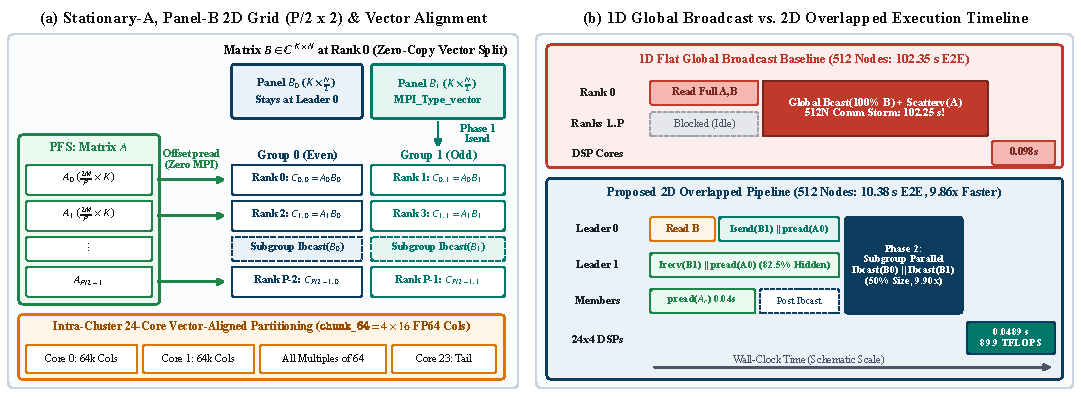
\includegraphics[width=0.68\textwidth]{fig2_2d_comm_timeline.pdf}
    \caption{Proposed Stationary-$A$, Panel-Broadcast-$B$ 2D hybrid orchestration ($P/2 \times 2$): (a) zero-copy strided \texttt{MPI\_Type\_vector} dispatch of $B$ panels, parallel \texttt{pread} of $A$, disjoint $C_{r,g}$ ownership, and 64-column partitioning; (b) asynchronous execution timeline contrasting 1D storm vs.\ 2D overlapped pipeline.}
    \label{fig:comm2d}
\end{figure*}

% ============================================================================
\section{Hierarchical 2D Data Orchestration}
\label{sec:host_2d}
% ============================================================================

\subsection{Stationary-$A$, Panel-Broadcast-$B$ Logical Grid}
A 1D broadcast baseline (\texttt{gemm\_host\_AS.c}) broadcasts $100\%$ of $B$ across all ranks, triggering network storms at 512 nodes ($102.25$~s). General $\sqrt{P} \times \sqrt{P}$ SUMMA~\cite{vandegeijn1997summa} incurs $\sqrt{P}$ iterative barriers, while 2.5D replication~\cite{solomonik2011comm25d} requires post-compute $C$ reductions and exceeds node RAM.

We formulate a $(P/G) \times G$ \textbf{Stationary-$A$, Panel-Broadcast-$B$ 2D grid} (Fig.~\ref{fig:comm2d}(a)). With $G=2$, rank $p \in [0, P-1]$ maps to subgroup $g = p \bmod G$, intra-group index $r = \lfloor p / G \rfloor$, and cluster $d = p \bmod 4$. Matrix $B$ is partitioned into $G$ vertical panels $B_g \in \mathbb{C}^{K \times N_g}$, while $A$ is partitioned into $P_g = P/G$ horizontal slices $A_r \in \mathbb{C}^{M_r \times K}$. Leader ranks ($r=0$) employ asymmetric load balancing: $M_0 = \lfloor M/P_g \rfloor$, shielding leaders from remainder rows. Each rank exclusively updates disjoint output $C_{r,g} \leftarrow C_{r,g} + A_r B_g$, requiring \textbf{zero network communication of $A$ and zero post-compute reduction of $C$}.

\begin{table}[t]
\centering
\caption{Asymptotic Per-Rank Complexity Across Distributed GEMM Schemes}
\label{tab:complexity}
\renewcommand{\arraystretch}{1.08}
\setlength{\tabcolsep}{3.0pt}
\resizebox{\columnwidth}{!}{%
\begin{tabular}{@{}lcccc@{}}
\toprule
\textbf{Distributed Scheme} & \textbf{Network Volume} & \textbf{Sync Stages} & \textbf{Local Rows} & \textbf{DDR-Streaming Floor} \\
\midrule
1D Flat Broadcast & $16 N^2 \log_2 P$ & 2 Global & $N / P$ & $\ge 16 N^2 / \mathcal{B}_{\mathrm{DDR}}$ \\
2D SUMMA ($\sqrt{P}$)~\cite{vandegeijn1997summa} & $\frac{32 N^2}{\sqrt{P}} \log_2 \sqrt{P}$ & $\frac{2N}{K_b} \log_2 \sqrt{P}$ & $N / \sqrt{P}$ & Stalls on Iterative Launches \\
2.5D ($c$ copies)~\cite{solomonik2011comm25d} & $\mathcal{O}(N^2 / \sqrt{P c})$ & Bcast + Reduce & $N \sqrt{c/P}$ & Extra $C$-Reduction Traffic \\
\textbf{Proposed 2D ($P/G \times G$)} & $\mathbf{\frac{16 N^2}{G} \log_2(P/G)}$ & \textbf{1 Subgroup} & $\mathbf{G N / P}$ & $\mathbf{\ge \frac{16 N^2}{G \cdot \mathcal{B}_{\mathrm{DDR}}}}$ (\textbf{$G\times$ Lower}) \\
\bottomrule
\end{tabular}%
}
\end{table}

\subsection{Zero-Copy Strided Vector Dispatch and Parallel \texttt{pread}}
To avoid copying $B_g$ into intermediate buffers at Rank~0, we commit a zero-copy strided datatype (\texttt{operator.c}):
\begin{equation}
\mathcal{D}_{B_g} \triangleq \texttt{MPI\_Type\_vector}(K,\; N_g,\; N,\; \texttt{MPI\_DOUBLE}),
\label{eq:mpi_vector}
\end{equation}
dispatching $B_g$ via non-blocking \texttt{MPI\_Isend} to subgroup leaders ($r=0, g \ge 1$), which unpack into contiguous DSP buffers via \texttt{MPI\_Irecv} (Phase~1). Leaders then execute non-blocking \texttt{MPI\_Ibcast} across isolated subgroup communicators $\mathcal{C}_g$ of size $P/G$ (Phase~2).

Concurrently, every rank $(r, g)$ invokes POSIX \texttt{pread64} at byte offset $\Delta_r = 8 \cdot i_0(r) \cdot K$ to stream its $A_r$ slice directly from storage into Hthread DMA-mapped memory, completely overlapping file I/O with Phase-1 network progress (Fig.~\ref{fig:comm2d}(b)).

\subsection{64-Column Vector Alignment and Optimality of $G=2$}
Distributing $N_g$ columns across $T=24$ DSP cores requires enforcing \textbf{64-column vector alignment} (\texttt{chunk\_64 = 64}): core $t$ receives $N_{\mathrm{thread}}(t) = 64(q + 1)$ for $t < u$, and $64 q$ otherwise ($Q = \lfloor N_g/64 \rfloor, q = \lfloor Q/24 \rfloor, u = Q \bmod 24$). For $N=8192$: (i) 24-core occupancy requires $N_g \ge 24 \times 64 = 1{,}536 \implies G \le 4$; (ii) 3-stage $C$-buffering requires $N_{\mathrm{thread}} \ge 3 N_b = 192$ columns, ruling out $G=4$ where 16 cores receive only 64 columns; (iii) $G=2$ ($N_g=4{,}096$) provides 192 columns to 16 cores and 128 to 8 cores with zero tail padding, uniquely satisfying all constraints.

\begin{table*}[t]
\centering
\caption{Intra-Node Performance (GFLOPS), Speedup, and FP64 Numerical Accuracy vs.\ Multi-Threaded ARMv8 OpenBLAS}
\label{tab:intra_node}
\renewcommand{\arraystretch}{1.06}
\setlength{\tabcolsep}{4.5pt}
\resizebox{\textwidth}{!}{%
\begin{tabular}{@{}rccccccccccc@{}}
\toprule
 & \multicolumn{4}{c}{\textbf{Single-Core Compute Density (1 Core)}} & \multicolumn{5}{c}{\textbf{Cluster-Level Throughput (1 DSP Cluster [24C] vs.\ CPU)}} & \multicolumn{2}{c}{\textbf{FP64 Max Error ($\ell_\infty$)}} \\
\cmidrule(lr){2-5} \cmidrule(lr){6-10} \cmidrule(l){11-12}
\textbf{Scale $N$} & \textbf{DSP 1C} & \textbf{CPU 1C} & \textbf{CPU 1C} & \textbf{Speedup} & \textbf{DSP 24C} & \textbf{CPU 4C} & \textbf{CPU 16C} & \textbf{vs.\ 4C} & \textbf{vs.\ 16C} & $\max|\Delta C_{\mathrm{Re}}|$ & $\max|\Delta C_{\mathrm{Im}}|$ \\
($M\!=\!N\!=\!K$) & \textbf{Ours} & \texttt{4xDGEMM} & \texttt{1xZGEMM} & (\texttt{4D} / \texttt{1Z}) & \textbf{(1 Clust.)} & \texttt{4xDGEMM} & \texttt{1xZGEMM} & (\textbf{Equiv}) & (\texttt{1Z}) & (Real Part) & (Imag Part) \\
\midrule
$512$ & \textbf{44.16} & 7.22 & 7.10 & $6.12\times$ / $6.22\times$ & \textbf{80.98} & 23.32 & 40.99 & $3.47\times$ & $1.98\times$ & $7.28\times 10^{-12}$ & $1.13\times 10^{-10}$ \\
$1{,}024$ & \textbf{45.77} & 7.07 & 7.69 & $6.48\times$ / $5.95\times$ & \textbf{139.73} & 28.38 & 82.29 & $4.92\times$ & $1.70\times$ & $1.73\times 10^{-11}$ & $3.27\times 10^{-10}$ \\
$2{,}048$ & \textbf{49.19} & 6.80 & 7.63 & $7.24\times$ / $6.45\times$ & \textbf{145.96} & 22.84 & 92.49 & $6.39\times$ & $1.58\times$ & $4.37\times 10^{-11}$ & $9.75\times 10^{-10}$ \\
$4{,}096$ & \textbf{48.39} & 6.78 & 7.74 & $7.13\times$ / $6.25\times$ & \textbf{173.05} & 24.41 & 85.51 & $7.09\times$ & $2.02\times$ & $7.46\times 10^{-11}$ & $2.79\times 10^{-9}$ \\
$8{,}192$ & \textbf{49.16} & 6.76 & 7.60 & $\mathbf{7.28\times}$ / $\mathbf{6.47\times}$ & \textbf{243.44} & 26.08 & 89.65 & $\mathbf{9.33\times}$ & $\mathbf{2.72\times}$ & $1.89\times 10^{-10}$ & $7.57\times 10^{-9}$ \\
$16{,}384^{\dagger}$ & \textbf{49.16} & 7.20 & OOM & $6.83\times$ / --- & \textbf{199.21} & 26.62 & OOM & $7.48\times$ & --- & $1.05\times 10^{-9}$ & $2.18\times 10^{-8}$ \\
\bottomrule
\end{tabular}%
}
\vspace{1pt}
\par{\raggedright\scriptsize $^{\dagger}$At $N=16384$, allocating 12 GiB AoS buffers alongside planar host buffers exceeds 32 GB node RAM; DSP evaluation executes via $2 \times 2$ host-tiled scheduling.\par}
\end{table*}

\begin{figure*}[t]
    \centering
    \begin{minipage}[t]{0.31\textwidth}
        \centering
        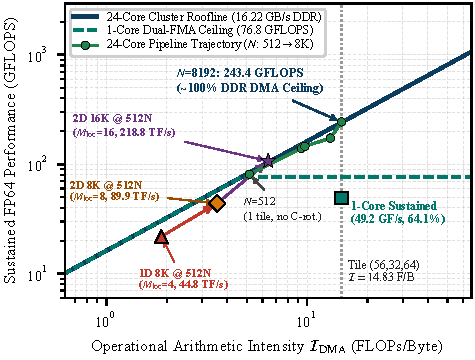
\includegraphics[width=\linewidth]{fig5_roofline_model.pdf}
        \caption{Empirical cluster Roofline model ($16.22$~GB/s DDR4 DMA ceiling) and 512-node trajectory.}
        \label{fig:roofline}
    \end{minipage}\hfill
    \begin{minipage}[t]{0.67\textwidth}
        \centering
        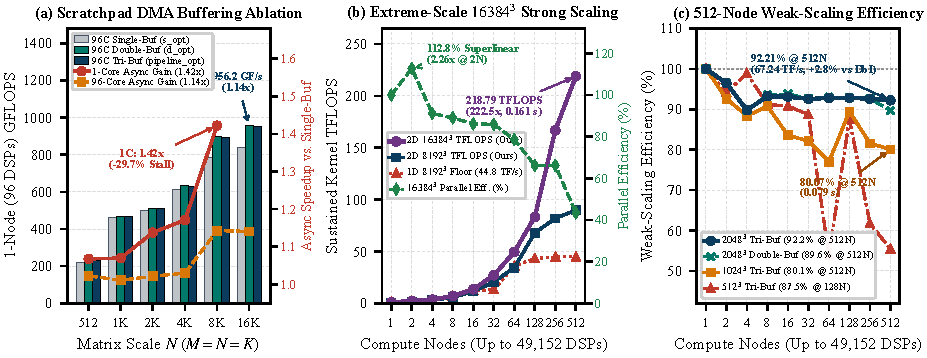
\includegraphics[width=\linewidth]{fig7_ablation_extreme_weak.pdf}
        \caption{Experimental scaling results: (a) DMA buffering ablation; (b) extreme $16384^3$ strong scaling to $218.79$~TFLOPS; (c) 1--512 node weak scaling maintaining $92.21\%$ efficiency across 49,152 DSP cores.}
        \label{fig:scaling}
    \end{minipage}
\end{figure*}

\begin{table*}[t]
\centering
\caption{Multi-Scale Distributed Strong and Weak Scaling Across 1 to 512 MT-3000 Nodes (4 to 2,048 MPI Ranks; 96 to 49,152 DSP Cores)}
\label{tab:strong_scaling}
\renewcommand{\arraystretch}{1.04}
\setlength{\tabcolsep}{3.2pt}
\resizebox{\textwidth}{!}{%
\begin{tabular}{@{}rrrcccccccccccc@{}}
\toprule
 & & & \multicolumn{7}{c}{\textbf{$8192^3$ Strong Scaling ($4.398$~TFLOPs)}} & \multicolumn{3}{c}{\textbf{Extreme $16384^3$ 2D Strong ($35.18$~TF)}} \\
\cmidrule(lr){4-10} \cmidrule(lr){11-13}
\textbf{Nodes} & \textbf{MPI} & \textbf{DSP} & \textbf{1D Kern.} & \textbf{1D TF/s} & \textbf{1D Comm} & \textbf{2D Kern.} & \textbf{2D TF/s} & \textbf{2D Comm} & \textbf{Gain} & \textbf{16K Kern.} & \textbf{16K TF/s} & \textbf{Weak TF/s} \\
 & \textbf{Ranks} & \textbf{Cores} & \textbf{(s)} & \textbf{(Eff.\ \%)} & \textbf{(s)} & \textbf{(s)} & \textbf{(Eff.\ \%)} & \textbf{(s)} & \textbf{(Kern / Comm)} & \textbf{(s)} & \textbf{(Eff.\ \%)} & \textbf{($2048^3$, Eff.\ \%)} \\
\midrule
1 & 4 & 96 & 4.5354 & 0.97 (100\%) & 9.01 & 5.7812 & 0.76 (100\%) & 2.89 & $0.78\times$ / $3.12\times$ & 35.7795 & 0.98 (100\%) & 0.14 (100\%) \\
2 & 8 & 192 & 2.3148 & 1.90 (97.9\%) & 13.94 & 2.8848 & 1.52 (100\%) & 5.09 & $0.80\times$ / $2.74\times$ & 15.8621 & 2.22 (\textbf{112.8\%}) & 0.28 (96.5\%) \\
4 & 16 & 384 & 1.2773 & 3.44 (88.7\%) & 18.02 & 1.4777 & 2.98 (97.8\%) & 7.10 & $0.86\times$ / $2.54\times$ & 9.8105 & 3.59 (91.2\%) & 0.51 (89.8\%) \\
8 & 32 & 768 & 0.6532 & 6.73 (86.7\%) & 18.88 & 0.7639 & 5.76 (94.6\%) & 7.70 & $0.86\times$ / $2.45\times$ & 5.0231 & 7.01 (89.0\%) & 1.06 (93.2\%) \\
16 & 64 & 1,536 & 0.3629 & 12.12 (78.1\%) & 20.28 & 0.3877 & 11.34 (93.2\%) & 9.73 & $0.94\times$ / $2.08\times$ & 2.5957 & 13.56 (86.2\%) & 2.12 (93.1\%) \\
32 & 128 & 3,072 & 0.3319 & 13.25 (42.7\%) & 24.26 & 0.2133 & 20.62 (84.7\%) & 8.33 & $\mathbf{1.56\times}$ / $2.91\times$ & 1.3007 & 27.05 (\textbf{86.0\%}) & 4.22 (92.6\%) \\
64 & 256 & 6,144 & 0.1222 & 36.00 (58.0\%) & 32.21 & 0.1284 & 34.26 (70.4\%) & 10.26 & $0.95\times$ / $3.14\times$ & 0.7112 & 49.47 (78.6\%) & 8.46 (92.8\%) \\
128 & 512 & 12,288 & 0.1017 & 43.24 (34.8\%) & 26.96 & 0.0647 & \textbf{68.01} (69.8\%) & 8.75 & $\mathbf{1.57\times}$ / $3.08\times$ & 0.4223 & 83.31 (66.2\%) & 16.92 (92.8\%) \\
256 & 1,024 & 24,576 & 0.0984 & 44.70 (18.0\%) & 36.02 & 0.0538 & \textbf{81.77} (42.0\%) & 10.43 & $\mathbf{1.83\times}$ / $3.45\times$ & 0.2109 & \textbf{166.82} (66.3\%) & 33.76 (92.6\%) \\
\textbf{512} & \textbf{2,048} & \textbf{49,152} & 0.0982 & 44.78 (9.0\%) & 102.25 & \textbf{0.0489} & \textbf{89.92} (23.1\%) & \textbf{10.32} & $\mathbf{2.01\times}$ / $\mathbf{9.90\times}$ & \textbf{0.1608} & \textbf{218.79} (43.5\%) & \textbf{67.24} (\textbf{92.2\%}) \\
\bottomrule
\end{tabular}%
}
\end{table*}

% ============================================================================
\section{Experimental Evaluation}
\label{sec:eval}
% ============================================================================
We evaluate our framework on the MT-3000 supercomputer scaling from 1 to 512 nodes (up to 2,048 MPI ranks and 49,152 bare-metal DSP cores, $5.94$~PFLOPS aggregate peak). Host code is compiled with \texttt{mpicc -O2 -fopenmp}; DSP code is built with the vendor VLIW/SIMD C compiler.

\subsection{Intra-Node Performance, Roofline, and Accuracy}
Table~\ref{tab:intra_node} and Fig.~\ref{fig:roofline} summarize intra-node evaluation:
\begin{itemize}\setlength{\itemsep}{0.5pt}\setlength{\parskip}{0pt}
    \item \textbf{Single-Core Throughput:} 1 DSP core sustains $44.16$--$49.19$~GFLOPS ($64.1\%$ of peak), outperforming 1-core OpenBLAS by $6.12\times$--$7.28\times$ (\texttt{4x DGEMM}) and $5.95\times$--$6.47\times$ (\texttt{1x ZGEMM}).
    \item \textbf{Cluster-Level Saturation:} 1 DSP cluster (24 cores) reaches \textbf{$243.44$~GFLOPS} at $N=8192$, matching our $240.5$~GFLOPS DDR4 Roofline ceiling within $1.2\%$ ($\sim\!100\%$ saturation). This outperforms 4-core CPU OpenBLAS by \textbf{$9.33\times$} and full 16-core CPU OpenBLAS by \textbf{$2.72\times$}. 1 full node (96 cores) achieves \textbf{$956.17$~GFLOPS} ($99.4\%$ of the 962.0 GFLOPS 4-cluster node Roofline).
    \item \textbf{DMA Buffering Ablation:} As shown in Fig.~\ref{fig:scaling}(a), asynchronous double buffering raises 1-core throughput from 33.79 to $48.05$~GFLOPS ($1.422\times$ speedup, $29.69\%$ runtime cut), and boosts 96-core node throughput from $838.03$ to $956.17$~GFLOPS ($1.141\times$).
    \item \textbf{FP64 Precision:} Across all scales, element-wise maximum error against OpenBLAS scales as $\mathcal{O}(K \epsilon_{\mathrm{FP64}})$ bounded within $7.28 \times 10^{-12}$ to $2.18 \times 10^{-8}$ (Table~\ref{tab:intra_node}), confirming fused FMA stability.
\end{itemize}

\subsection{Multi-Scale Distributed Strong and Weak Scaling}
Table~\ref{tab:strong_scaling} and Fig.~\ref{fig:scaling}(b)(c) report 1- to 512-node results:
\begin{itemize}\setlength{\itemsep}{0.5pt}\setlength{\parskip}{0pt}
    \item \textbf{$8192^3$ Strong Scaling:} At 512 nodes, 1D stalls at the DDR streaming floor ($44.78$~TFLOPS) while broadcast latency explodes to $102.25$~s. Our 2D co-design restricts communication to $10.32$~s (\textbf{$9.90\times$ speedup}) and doubles kernel throughput to \textbf{$89.92$~TFLOPS ($2.01\times$ speedup)}, validating~\eqref{eq:ddr_floor}. Concurrent \texttt{pread} accelerates member I/O by up to $93.5\times$ and hides $82.5\%$ of leader I/O.
    \item \textbf{Extreme $16384^3$ Strong Scaling:} Workload scaling ($35.184$~TFLOPs) achieves \textbf{$112.80\%$ superlinear efficiency} at 2 nodes by halving cache/memory pressure, sustains $66.26\%$ efficiency at 256 nodes ($166.82$~TFLOPS), and delivers \textbf{$218.79$~TFLOPS} ($0.1608$~s, $222.49\times$ speedup) at 512 nodes ($49{,}152$ DSPs), closely matching our theoretical prediction of 212.3 TFLOPS.
    \item \textbf{512-Node Weak Scaling:} Under $2048^3$ base workload ($68.72$~GFLOPs/node), runtime rises by just $40.7$~ms across a $512\times$ scale-out ($0.4825 \to 0.5233$~s), maintaining \textbf{$92.21\%$ efficiency ($67.24$~TFLOPS)} at 49,152 DSP cores. Triple buffering provides $+2.77\%$ higher throughput over double buffering by absorbing memory/NIC jitter.
\end{itemize}

% ============================================================================
\section{Related Work}
\label{sec:related}
% ============================================================================
\subsection{Scratchpad Co-Design and Software DMA Scheduling}
Replacing hardware cache hierarchies with software-managed scratchpad memories (SPMs) eliminates cache tag overhead, coherence protocol traffic, and cache conflict misses, delivering higher energy efficiency and predictable execution~\cite{kahle2005cell, igual2012dsp, fu2016sunway}. Early pioneers such as the IBM Cell Broadband Engine~\cite{kahle2005cell} utilized memory flow controllers (MFC) to stage tiles across 256~KB local stores. The Sunway SW26010 architecture~\cite{fu2016sunway, jiang2017sw26010} integrates 64~KB local data memory (LDM) per core, coordinating register communication buses for matrix multiplication. Modern spatial accelerators such as Tenstorrent, Cerebras CS-2, and Google TPU similarly rely on explicit SRAM tiling. Prior MT-3000 studies optimized real-valued GEMM, stencils, or attention mechanisms on single nodes~\cite{lu2022mt3000, li2024md, fang2026mtgemm, mo2024irregular, qi2025constraint, qi2026attention}. Our work differs fundamentally by addressing double-precision complex ZGEMM on an asymmetric dual-scratchpad architecture (64~KB SM + 768~KB AM), establishing a 14-channel tri-buffered DMA pipeline that hides bidirectional $C$-tile write-back latencies while pinning 32 vector registers for zero compiler spilling.

\subsection{Dense Complex Linear Solvers in EDA Applications}
Double-precision complex GEMM is the foundational computational kernel in large-scale electronic design automation (EDA), including full-wave electromagnetic boundary element methods (Method of Moments, MoM) for on-chip parasitic extraction, antenna array simulation, high-speed interconnect modeling, and quantum circuit state evolution~\cite{barrett2010complexhpl, vanzee2017complex}. Standard open-source BLAS libraries such as OpenBLAS~\cite{zhang2012openblas} and BLIS~\cite{vanzee2015blis, vanzee2017complex} are heavily tuned for multi-level CPU cache hierarchies and rely on Array-of-Structures (AoS) layouts, which induce prohibitive vector lane shuffling overheads on wide 16-lane SIMD engines. Furthermore, algebraic 3M algorithms~\cite{vanzee2017complex} reduce nominal FLOP counts but demand extensive workspace allocations and suffer $\mathcal{O}(\kappa)$ numerical cancellation~\cite{higham2002accuracy}. Our planar split-complex 4M formulation avoids auxiliary memory while preserving full IEEE FP64 precision across all matrix dimensions.

\subsection{Communication-Avoiding Distributed Matrix Multiplication}
Distributed dense matrix multiplication has been extensively studied on cache-based homogeneous clusters. Canonical 2D SUMMA~\cite{vandegeijn1997summa} and ScaLAPACK~\cite{choi1996scalapack} broadcast sub-blocks in $\mathcal{O}(\sqrt{P})$ algorithmic steps, introducing fine-grained synchronization overheads. 2.5D GEMM~\cite{solomonik2011comm25d} and 3D algorithms reduce communication by replicating input matrices $c$ times, but require post-computation global reductions of the $C$ matrix and exceed per-node memory budgets at large scale. Recent communication-optimal frameworks such as COSMA~\cite{kwasniewski2019cosma} and SLATE~\cite{gates2019slate} optimize tile shapes for cache-coherent CPU/GPU systems but assume transparent hardware prefetching and symmetric interconnects. Our Stationary-$A$, Panel-Broadcast-$B$ ($P/2 \times 2$) scheme completely avoids network communication of $A$ and post-compute reductions of $C$, eliminates buffer packing via committed \texttt{MPI\_Type\_vector} strided datatypes, overlaps parallel POSIX \texttt{pread} with non-blocking P2P dispatch, and halves the off-chip DDR-streaming floor at extreme supercomputer scale.

% ============================================================================
\section{Conclusion}
\label{sec:conclusion}
% ============================================================================
We presented an end-to-end hardware-software co-design framework for distributed double-precision complex GEMM on multi-zone heterogeneous DSP supercomputers. By coupling an intra-chip 14-channel asynchronous DMA tri-buffered pipeline and a $4 \times 4$ register-resident dual-FMA micro-kernel with an inter-node Stationary-$A$, Panel-Broadcast-$B$ 2D hybrid orchestration, our solution breaks both the on-chip scratchpad memory wall and the inter-node network communication wall. Single-core throughput reaches $49.19$~GFLOPS ($64.1\%$ peak), cluster throughput achieves $243.44$~GFLOPS ($\sim\!100\%$ Roofline saturation), and node throughput reaches $956.17$~GFLOPS. Scaling to 512 MT-3000 nodes (2,048 MPI ranks, 49,152 DSP cores), our framework reduces collective communication time by $9.90\times$, doubles kernel throughput to $89.92$~TFLOPS ($8192^3$), delivers $218.79$~TFLOPS on extreme $16384^3$ workloads ($222.49\times$ speedup, $112.80\%$ 2-node superlinear efficiency), and sustains $92.21\%$ weak-scaling efficiency. This co-design establishes a viable blueprint for deploying memory- and communication-intensive dense linear algebra solvers on next-generation heterogeneous accelerator architectures.

\clearpage
\IEEEtriggeratref{14}
\bibliographystyle{IEEEtran}
\bibliography{references}

\end{document}
